
\subsection{Radianai}
Radianas - kampo dydžio matavimo vienetas. \textbf{Gali} būti žymimas: $rad$.

\begin{math} \\
    1rad = \frac{180}{pi}\degree \approx 57 \degree \\
    1\degree = \frac{pi}{180}
\end{math}

\subsection{Trigonometrinės funkcijos}
Trigonometrinės funkcijos yra $\sin$, $\cos$, $\tg$, $\ctg$, $\arcsin$ ir daugiau\dots
Jos gali būti naudojamos išmatuoti smailųjį kampą stačiajame trikampyje, daugelyje formulių ir t.t\dots

\subsection{Statieji trikampiai}
{
\begin{wrapfigure}{l}{0.4\textwidth}
\caption{\textit{Iliustracijos -- tiek reikalingos, kiek nuobodžios daryti.}}
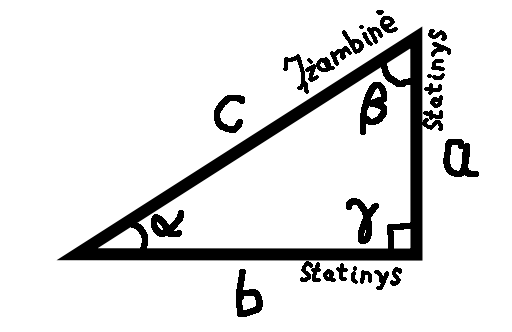
\includegraphics[scale=0.5]{right_triangle.png}
\end{wrapfigure}

\begin{equation*} \\
    \begin{aligned}[c]
        \sin \alpha &= \frac{a}{c} \\
        \cos \alpha &= \frac{b}{c} \\
        \tg  \alpha &= \frac{a}{b} \\
        \ctg \alpha &= \frac{b}{a}
    \end{aligned}
    \hspace{10mm}
    \begin{aligned}[c]
        c^2 &= a^2 + b^2 \\
        S &= \frac{ab}{2}
    \end{aligned}
\end{equation*}
}

\clearpage
\subsection{Įvairiakraščiai trikampiai}

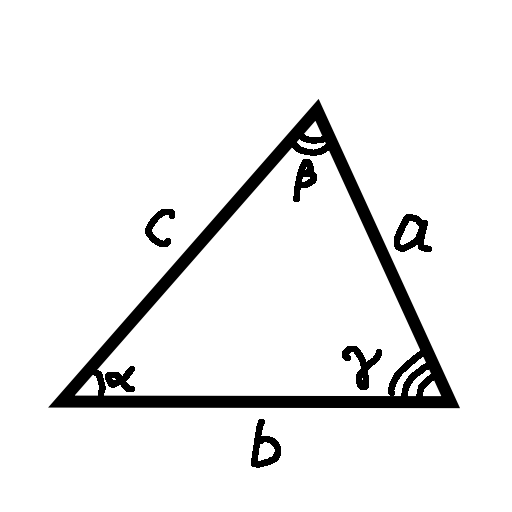
\includegraphics[scale=0.5]{icocele_triangle.png}

\begin{equation*}
    \begin{aligned}[c]
        180\degree &= \alpha + \beta + \gamma \\
        \frac{a}{\sin \alpha} &= \frac{b}{\sin \beta} = \frac{c}{\sin \gamma} \\
        a^2 &= b^2 + c^2 - 2\, b\, c\,\cos \alpha \\
        S &= \frac{a\,b}{2} \cdot \sin \gamma
    \end{aligned}
    \hspace{40mm}
    \begin{aligned}[c]
        \textit{Sinuso\ teorema} \\
        \textit{Kosinuso\ teorema} \\
    \end{aligned}
\end{equation*}


\subsection{Trigonometrinės formulės}

\begin{equation*} \\
    \begin{aligned}[c]
        \sin(\alpha \pm \beta) &= \sin\alpha\cos\beta \pm \sin\beta\cos\alpha \\
        \cos(\alpha \pm \beta) &= \cos\alpha\cos\beta \mp \sin\alpha\sin\beta \\
        \tg (\alpha \pm \beta) &= \frac{\tg\alpha \pm \tg\beta}{1 \mp \tg\alpha \tg\beta} \\ \\
        \sin(2\alpha) &= \sin(\alpha + \alpha) = 2\sin\alpha\cos\alpha \\
        \cos(2\alpha) &= \cos(\alpha + \alpha) = \cos^2\alpha - \sin^2\alpha
    \end{aligned}
    \hspace{20mm}
    \begin{aligned}[c]
        \sin{\alpha}^2 + \cos{\alpha}^2 &= 1 \\
        \tg \alpha \cdot \ctg \alpha &= 1 \\
        \tg \alpha &= \frac{\sin \alpha}{\cos \alpha} \\
        \ctg \alpha &= \frac{1}{\tg \alpha} \\
        1 + \tg^2 \alpha &= \frac{1}{\cos^2 \alpha} \\  
        1 + \ctg^2 \alpha &= \frac{1}{\sin^2 \alpha} \\  
    \end{aligned}
\end{equation*}

\subsubsection{Pratimai}

\begin{exercises} \\
    \item $\ctg 30\degree               $
    \item $\ctg(45\degree + 45\degree)  $
    \item $\sin 75\degree               $
    \item $\cos( \alpha - 90\degree )   $
    \item $\tg \alpha\ ((\tg\alpha\ (\tg \alpha + \ctg \alpha))^{-1}\ - 1) $ 
\end{exercises} 

\subsubsection{Daugiau}

\begin{math}
    \sin(10\cdot 30\degree) = \sin(30\degree + 9 \cdot 30\degree) = \\
    \sin 30\degree \cos 30\degree + \sin(9 \cdot 30\degree)\cos(9 \cot 30\degree) = \\
    \frac{\sqrt{3}}{4} + \sin(30\degree + 8 \cdot 30\degree)\cos(30\degree + 8 \cdot 30\degree) = ... \\ 
    \\
    \sin(10 \cdot 30\degree) = \sin(300\degree) \Rightarrow 
    \sin(300\degree - 270\degree) \Rightarrow -\cos(30\degree) = -\frac{\sqrt{3}}{2}
\end{math} \\

\begin{math} \\
    \tg(\alpha + \beta) = \frac{\sin(\alpha + \beta)}{\cos(\alpha + \beta)}
\end{math}

\subsection{Redukcija}

Redukcija yra naudojama norint gauti tikslią $\sin, \cos, \tg$ ar $\ctg$ reikšmę iš lentelės (kurioje reikšmes yra nuo $0$ iki $90\degree).$ Redukcija veikia dėl sinusoidės ir kosinusoidės simetriškumo.\\

Trig. funkcijų periodai$(T)$: $T_{sin} = 360\degree, T_{cos} = 360\degree, T_{tg} = 180\degree, T_{\ctg} = 180\degree $

$\sin(\alpha + 90\degree) = \cos\alpha$
\begin{enumerate}
    \item Jei $\alpha > T$, \\
        $\alpha \Rightarrow \alpha \mod T$, \textit{arba atimti $T$ iš $\alpha$, kol $\alpha < T$}
    \item Jei $\alpha \ge 90\degree$, žiūrėti pagal ketvirčius: \\
        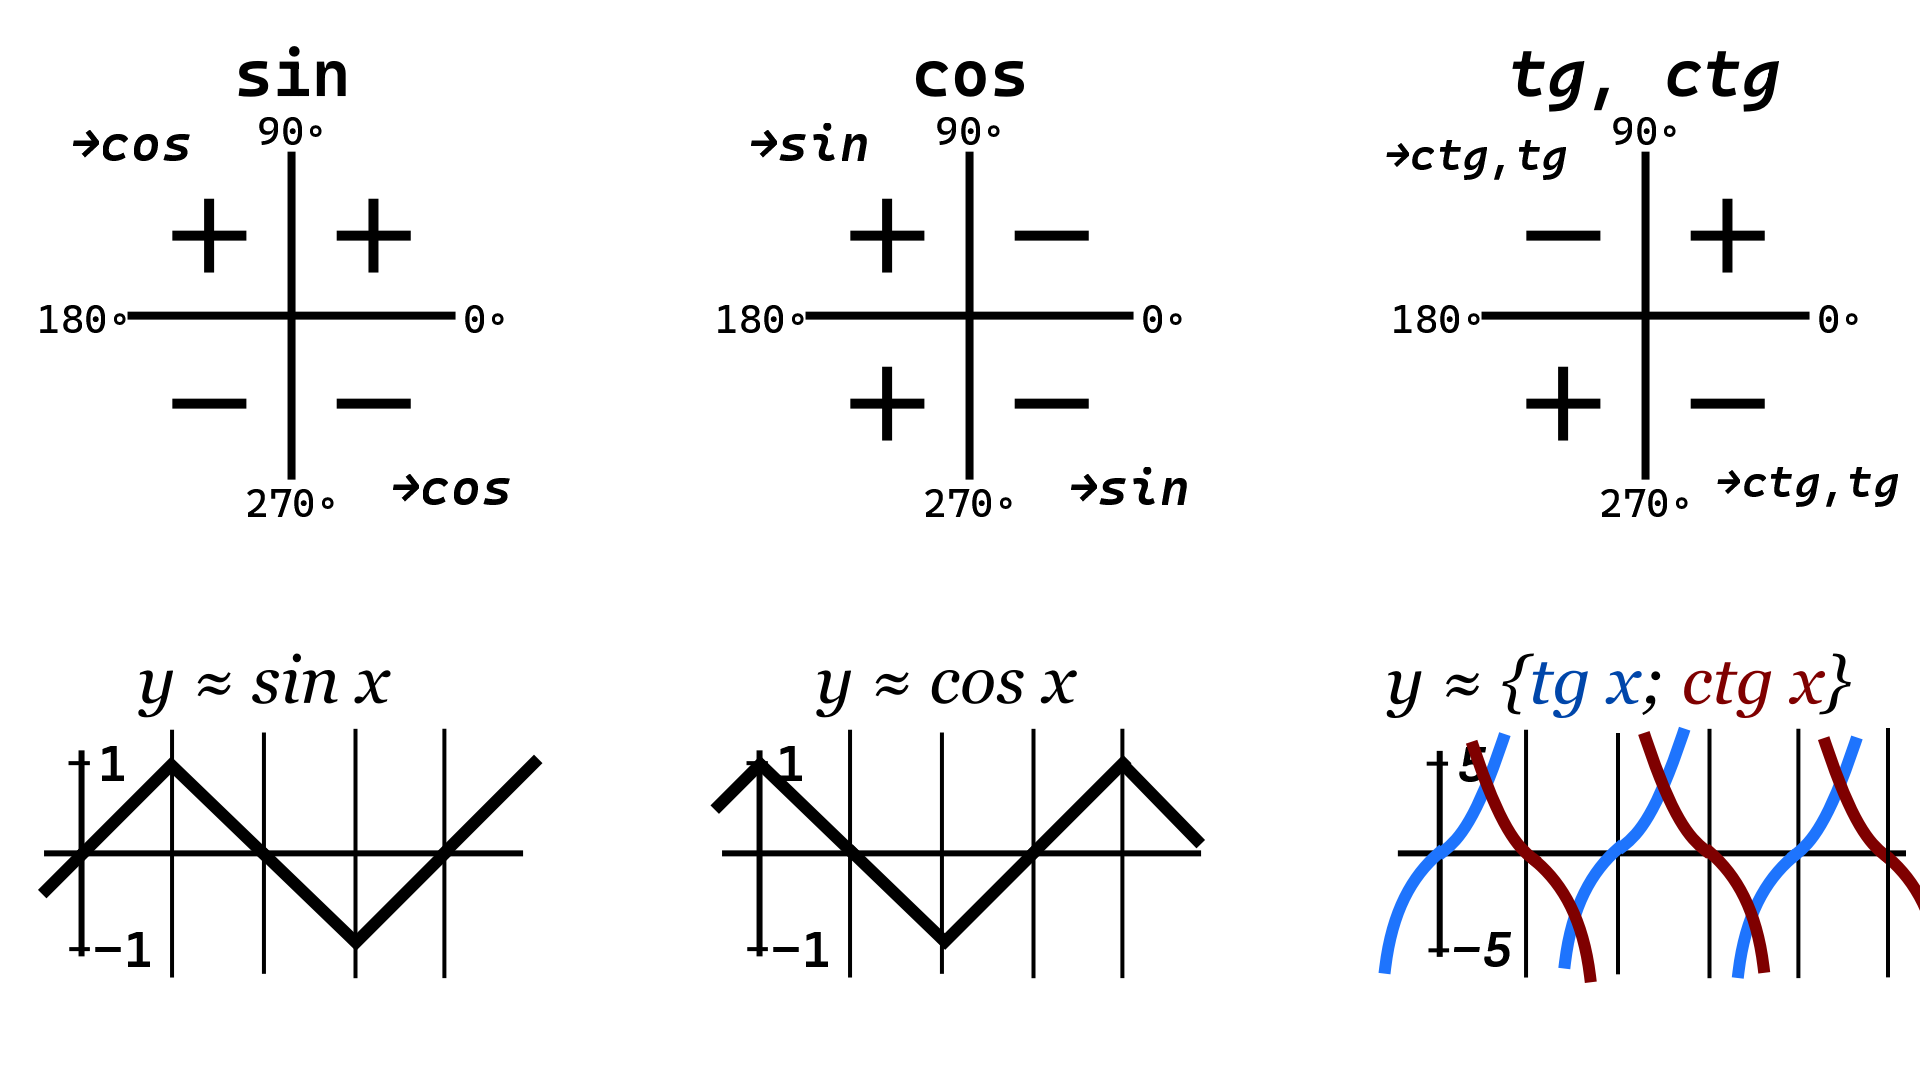
\includegraphics[scale=0.25]{assets/reduction.png} 
    \item Jei $\alpha \le 90\degree$, \\
        tikslią trig. funkcijos reikšmę galima rasti lentelėje.

\end{enumerate}

\subsubsection{Pratimai}

\begin{exercises}
    \item $\sin 30\degree         $
    \item $\cos 30\degree         $
    \item $\sin 270\degree        $
    \item $\tg  300\degree        $ 
    \item $\ctg 120\degree        $
    \item $\sin 720\degree n, n \in \mathbb{Z} $
    \item $\sin(-45\degree) $
\end{exercises} 


\subsubsection{Daugiau}

\begin{table}[h]
    \begin{tabular}{|c|ccccccccc|} 
        % There has got to be a better way to do this, but I don't care right now
        \hline
        $\alpha,\,\degree$ & 0 & 30 & 45 & 60 & 90 & 120 & 135 & 150 & 180 \\ 
        \hline
        $\sin \alpha$ & 0 & $\frac{1}{2}$ & $\frac{\sqrt{2}}{2}$ & $\frac{\sqrt{3}}{2}$ & 1 
                      & $\frac{\sqrt{3}}{2}$ & $\frac{\sqrt{2}}{2}$ & $\frac{1}{2}$ & 0 \\
        \hline
    \end{tabular}
    \\ \\ \\
    \begin{tabular}{|c|cccccccc|}
        \hline
        $\alpha,\,\degree$ & 210 & 225 & 240 & 270 & 300 & 330 & 345 & 360 \\ 
        \hline
        $\sin \alpha$ & $-\frac{1}{2}$ & $-\frac{\sqrt{2}}{2}$ & $-\frac{\sqrt{3}}{2}$ & -1
                      & $-\frac{\sqrt{3}}{2}$ & $-\frac{\sqrt{2}}{2}$ & $-\frac{1}{2}$ & 0 \\
        \hline
    \end{tabular}
    \caption{Pratęsta $\sin \alpha$ lentelė}
\end{table}


\subsection{Atvirkštinės trigonometrinės funkcijos (arc-funkcijos).}

\begin{equation}
    \begin{aligned}[c]
        \sin(\arcsin a) &= a, & \arcsin x &= y,\,kai\ -1 \le x \le 1\ ir\ y \in \left[ -\frac{\pi}{2}; \frac{\pi}{2}\right] \\
        \cos(\arccos a) &= a, & \arccos x &= y,\,kai\ -1 \le x \le 1\ ir\ y \in \left[0;\pi\right] \\
        \tg (\arctg  a) &= a, & \arctg  x &= y,\,kai\ y \in \left[ -\frac{\pi}{2}; \frac{\pi}{2}\right]\\
        \ctg(\arcctg a) &= a, & \arcctg x &= y,\,kai\ y \in \left[0;\pi\right]
    \end{aligned}
\end{equation}

\begin{equation}
    \begin{aligned}[c]
        \sin x &= y, & x &= (-1)^n + \arcsin y + \pi{n}, n \in \mathbb{Z} \\
        \cos x &= y, & x &= \pm \arccos y + 2\pi{n}, n \in \mathbb{Z} \\
        \tg  x &= y, & x &= \arctg y + \pi{n}, n \in \mathbb{Z} \\
        \ctg x &= y, & x &= \arcctg y + \pi{n}, n \in \mathbb{Z} \\
    \end{aligned}
\end{equation}

\begin{equation}
    \left.
    \begin{aligned}[c]
        \sin x &= -1, & x &= -\frac{\pi}{2} &+\ 2\pi{n} \\
        \sin x &=  0, & x &=                &    \pi{n} \\
        \sin x &=  1, & x &= +\frac{\pi}{2} &+\ 2\pi{n}
    \end{aligned}
    \hspace {15mm}
    \begin{aligned}[c]
        \cos x &= -1, & x &= \pi            &+\ 2\pi{n} \\
        \cos x &=  0, & x &= \frac{\pi}{2}  &    \pi{n} \\
        \cos x &=  1, & x &=                &+\ 2\pi{n}
    \end{aligned}
    \hspace{5mm}
    \right\}
    n \in \mathbb{Z}
\end{equation}

\subsubsection{Daugiau}

$\arcsin x = y$, $y \in [-\frac{\pi}{2}; \frac{\pi}{2}]$, o ne, pavyzdžiui: $y \in [-\pi; \pi]$, nes y tūrėtų 2 atsakymus, būtų aibė $y = \{x_1; x_2\}$.

% \includegraphics[scale=0.5]{assets/arcsin_restriction_reason.png} TODO, oops

